% Here goes the introduction to Li-ion Batteries (LIBs). This includes the discussion of the topics mentioned in the introduction and graphs about co2 emission and the role of transportation sector in it.

The Earth stands at a critical juncture in its history, where the consequences of human activity on the environment have reached a crossroads of global significance. Climate change, driven primarily by the relentless emission of greenhouse gases, has manifested itself in increasingly severe weather patterns, rising sea levels, and ecological disruptions. The urgency of the situation cannot be overstated, as nations grapple with the complex challenge of reducing carbon dioxide (CO$_2$) emissions to mitigate the impending climate crisis \cite{solomon2009irreversible}. 

The transportation sector emerges as a critical contributor to the climate change predicament \cite{iea-transport}. As societies evolve and the global population continues to grow, the demand for transportation, particularly in the form of automobiles and other fossil-fuel-reliant means, has risen dramatically. 

\begin{figure}[h]
    \centering
    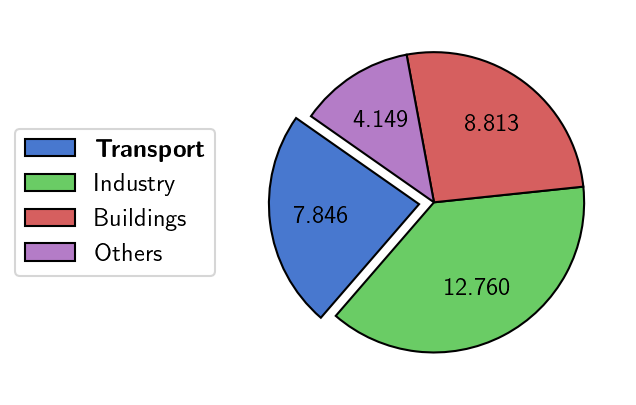
\includegraphics[width=0.7\textwidth]{Images/Chapter1/iea-transport.png}
    \caption{Global CO$_2$ emissions by sector. Source: IEA (2023) \cite{iea-transport}.}
    \label{fig:iea-transport}
\end{figure}


% \begin{figure}
%     \centering
%     
\includegraphics[width=0.7\textwidth]{Images/Chapter1/noaa-co2.png}
%     \caption{Trends in Atmospheric Carbon Dioxide. Source: NOAA (2023) \cite{noaa-co2}.}
%     \label{fig:noaa-co2}
% \end{figure}


% The dire need for sustainable energy solutions has never been more evident. While various sectors of the economy are challenged to reduce their carbon footprint, the transportation sector presents a unique dilemma. As people's mobility requirements persist, innovative solutions are crucial to decouple the connection between personal mobility and CO2 emissions. Electric vehicles (EVs) have emerged as a promising alternative to traditional internal combustion engine vehicles. They offer the potential to revolutionize the way we commute, significantly diminishing the transportation sector's contribution to carbon emissions. 

% At the heart of the electric vehicle industry's transformation lies lithium-ion batteries. These energy storage devices have rapidly gained prominence as the primary means of powering EVs. The suitability of lithium-ion batteries for this role is driven by their impressive energy density, rechargeability, and relatively low environmental impact compared to conventional fossil fuels. As we explore the potential of lithium-ion batteries, it becomes evident that their development and adoption may hold the key to mitigating the environmental impact of the transportation sector. 

% Lithium-ion batteries offer several key advantages that make them a compelling solution to the challenge of reducing CO$_2$ emissions in the transportation sector. Their high energy density allows electric vehicles to cover significant distances on a single charge, meeting the practical demands of modern commuting. Their rechargeability ensures that these batteries can be reused, reducing waste and minimizing their environmental footprint. Furthermore, the manufacturing and disposal of lithium-ion batteries have a comparatively lower impact on the environment when compared to the extraction and combustion of fossil fuels.

\section{Overview}
\label{sec:overview}

\subsection{Anode}
\label{sec:anode}

\subsection{Cathode}
\label{sec:cathode}

\subsection{Electrolyte}
\label{sec:electrolyte}

\subsection{Separator}
\label{sec:separator}

\subsection{Current Collectors}
\label{sec:current-collectors}

\subsection{Cell Geometries and Designs}
\label{sec:cell-geometries-designs}

\section{Safety and Degradation}
\label{sec:safety-degradation}
